\chapter{Definitions}
\label{chap:definitions}

\section{Brain Computer Interfaces}

Brain Computer Interfaces, abbreviated to \emph{BCI} and sometimes called Brain Machine Interfaces (in that case shortened to \emph{BMI}) are systems which consist of hardware and software systems which allow operation of external devices and computers by using only brain activity \cite{lebedev-2006}.

The way of acquisition of the brain signals differs from BCI to BCI and allows categorization into two main groups:
\subsection{Invasive BCI}
\label{sec:def:invasive}
Invasive BCI aim to use the signals from groups of single neurons or from groups of single neurons at multiple locations inside the brain \cite{lebedev-2006}. As the skull significantly interferes with signal quality when recording outside of the brain \cite{waldert-2016}, invasive BCIs use electrodes that are placed directly inside or on top of the brain itself (see Fig. \ref{def:bciLoc}). 
Providing optimal signal resolution with low noise, these kinds of BCIs find their applications in fields like controlling prostheses thus potentially restoring motor functions in patients \cite{waldert-2016}.

\begin{figure}[H]
    %\hspace*{-1.0cm}
    \centering
    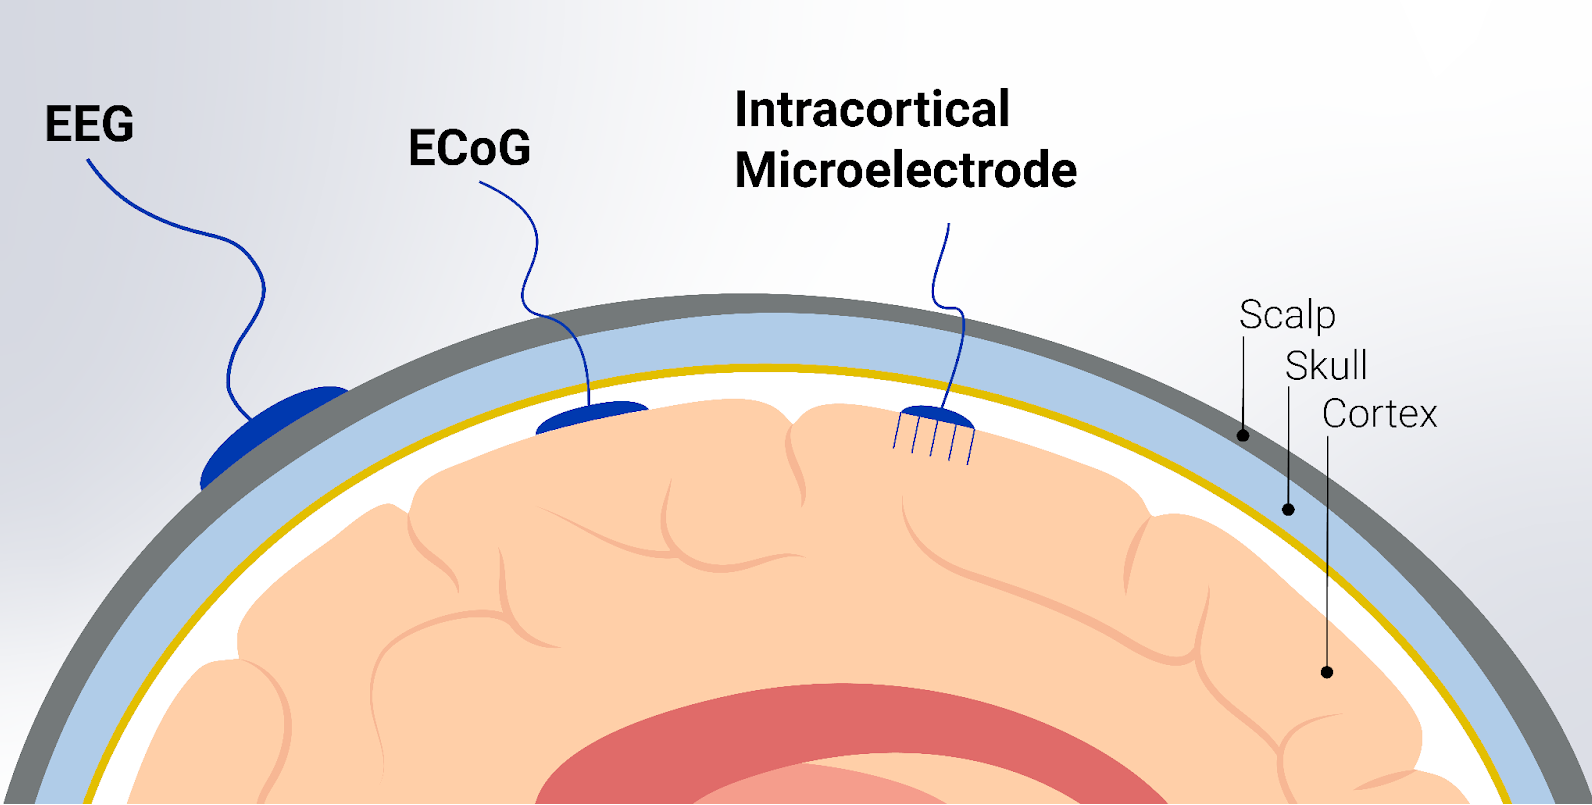
\includegraphics[scale=0.35]{gfx/SuI3_BCI_locations.PNG} 
    \caption{Overview over different recording sites of BCIs \cite{ONLINE:BCI_LOC}}
    \label{def:bciLoc}
\end{figure}

However, despite showing optimal signal quality for their applications, having these kind of BCIs come with some big disadvantages. The first and most obvious one is that a surgical procedure is required to insert the electrodes under the skull and on top or inside the brain, bringing the complications of surgery and recovery from such a procedure with it \cite{zhao-2023}. 
Furthermore, having any device placed on the brain with a surgical procedure requires greater reliability of the implanted device, which, in turn, not only makes the updates to the hard and software of invasive BCIs more complex but also significantly increases their overall cost \cite{zhao-2023}.

\subsection{Non-Invasive BCI}
\label{sec:def:non-invasive}

Non-invasive BCIs are BCIs that do not require any surgical procedure for collection of the required brain signals, which also presents as their most important advantage over the invasive BCI. Typically, the electrodes for measuring the brain activity are placed on top of the head where, in the case of using so called \emph{wet electrodes}, they are connected to the human scalp using a conductive gel to ensure stable electrical transmission.
\emph{Dry electrodes}, on the other hand, do not use any form of conductive gel and are instead placed directly on the scalp \cite{usakli2010improvement, yadav-2020}. 
To hold the electrodes in position for recording and to ensure they remain connected to the head during possible movement, they are usually placed on a so-called electrode caps, which feature preset openings for the electrodes to fit in (see Fig. \ref{def:bciNonInv}) \cite{usakli2010improvement}.

\begin{figure}[h]
    \hspace*{-0.0cm}
    \centering
    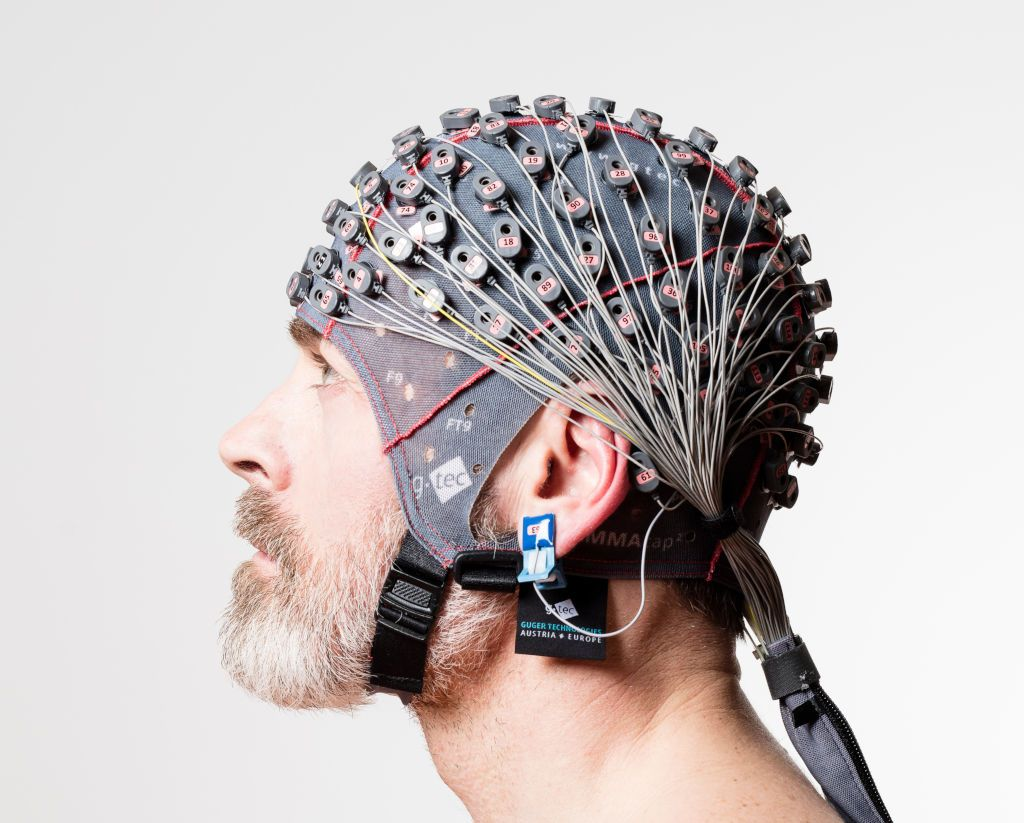
\includegraphics[scale=0.3]{gfx/SuI3_non_invasive_bci_gtec.jpg} 
    \caption{Example for electrode placement in non-invasive BCIs \cite{ONLINE:BCI_NIV}}
    \label{def:bciNonInv}
\end{figure}

While not needing surgery to be used, the recorded brain signals from non-invasive BCIs mainly suffer from lowered signal resolution and error sources (so-called \emph{artefacts}) such as movement, eye and noise artefacts \cite{waldert-2016}.
Other disadvantages and challenges of non-invasive BCI, including those specific to their use in gaming applications are discussed later in this paper in Chap. \ref{chap:challenges}.


\section{Frequency bands}
\label{sec:def:freqBand}

Brain signals tend to vary in frequency depending on what mental state the mind finds itself. The frequencies are summarised into so-called ``frequency bands'', which are listed and briefly explained in the following list, based on the one provided by Yadav et al. in their recent review of BCIs \cite{yadav-2020}:

% maybe turn into table?
\begin{itemize}
    \item \textbf{Delta} (\emph{1 - 3 Hz}): Normally only occur during deep sleep
    \item \textbf{Theta} (\emph{4 - 7 Hz}): Occur during sleep, drowsy or meditation states
    \item \textbf{Alpha} (\emph{7 - 12 Hz}): Occur while the brain is in a relaxed state
    \item \textbf{Beta} (\emph{12 - 30 Hz}): Occur during active thinking, concentration and alertness
    \item \textbf{Gamma} ( > 30 Hz): Occur while brain is processing and recognising external stimuli such as touch or sound
\end{itemize}

\section{BCI paradigms}
\label{sec:def:paradigm}

There are several established ways to acquire brain signals to be able to operate BCIs, summarised under the term of ``BCI paradigms''. These BCI paradigms can be differentiated according to whether they require an external stimulus (event-related potentials) for  operation or work without needing one (spontaneous potentials). 

\subsection{P300 signals}

A special % and widely used? can we back that up?
kind of Event-Related Potential (ERP) come in the form of the so-called ``P300 evoked potentials''. These potentials occur in reaction to a rarely occurring stimulus among an array of regular and systematic stimuli, termed ``oddball stimulus''. % cite
Such a potential can be triggered by asking a user to concentrate on a letter of their choice in a given matrix of letters on a computer screen (see Fig. \ref{def:P300}) while the computer randomly flashes through all of the available entries of the matrix individually. Approximately 300 ms after the chosen letter of the user is then randomly flashed, a potential can be registered in the brain activity of the user and thus said flashed letter can be correctly attributed to the letter the user chose to think about and concentrate on. Furthermore, it has been reported that the less likely the stimulus is, the higher the amplitude of the signal elicited by the oddball stimulus is. %cite!
% add sth about that it's not really usable for our cases? could then say that it might pose an accurate way to maybe move a character in an environment but is faaaar to slow for real use

\begin{figure}[H]
    \hspace*{-1.0cm}
    \centering
    
\includegraphics[scale=0.5]{gfx/MThes_P300Matrix.png} 
    \caption{Example of a P300 letter matrix used to mentally type out words for the computer to  voice out \cite{farwell-1988}}
    \label{def:P300}
\end{figure}



\subsection{Steady-State Visually Evoked Potentials (SSVEPs)}

Steady-State Visually Evoked Potentials (SSVEPs) are a particular kind of Evoked Potentials (EPs), which themselves are a subset of ERPs. EPs are potentials which can be recorded when the brain is focusing attention on an external stimulus, like a visual or auditory stimulus and show different characteristics based on the used stimulus \cite{martisius-2016}. 

Visual EPs, which are used in SSVEPs, feature a certain characteristic that makes them highly useful for controlling BCIs: When presented with a visual stimulus in the form of a flickering light source, the potential which is evoked shows the exact same frequency as the flickering light source (See Fig. \ref{def:VEP}) \cite{martisius-2016}.

\begin{figure}[H]
    \hspace*{-1.0cm}
    \centering
    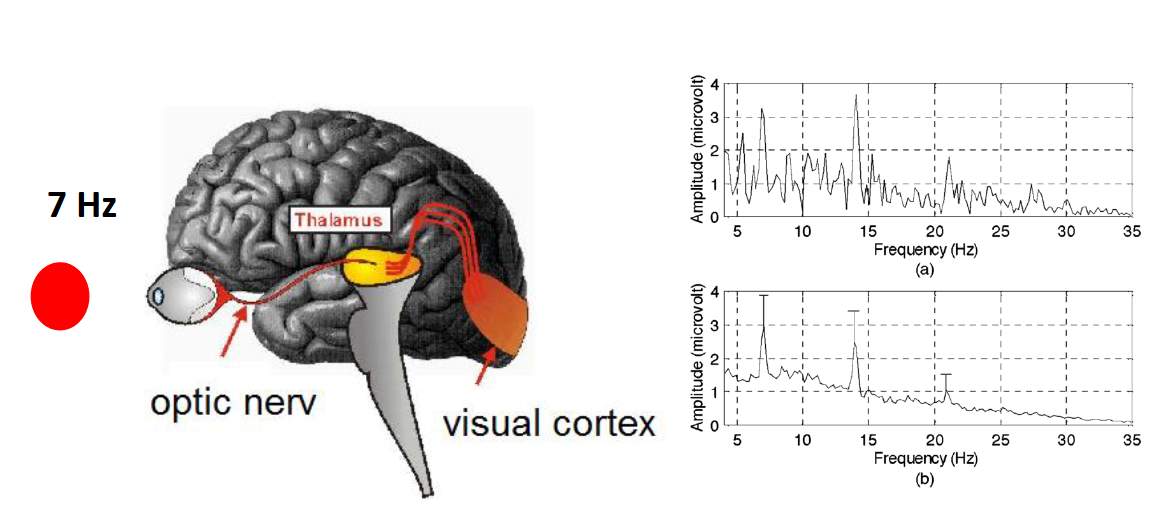
\includegraphics[scale=0.5]{gfx/SuI3_VEP.PNG} 
    \caption{Effects of a flickering light source on the resulting VEP frequency (based on \cite{IMG:VEP})}
    \label{def:VEP}
\end{figure}

SSVEPs use this effect to show multiple flickering light sources, each flickering at their own distinct frequency, to determine which light source the user is currently focusing their attention on at any given moment. This allows a clear classification of the resulting neural responses, as opposed to the area estimation of the regional brain activity evoked during spontaneous potentials. \cite{martisius-2016}. % rephrase?

\begin{figure}[H]
    \hspace*{-1.0cm}
    \centering
    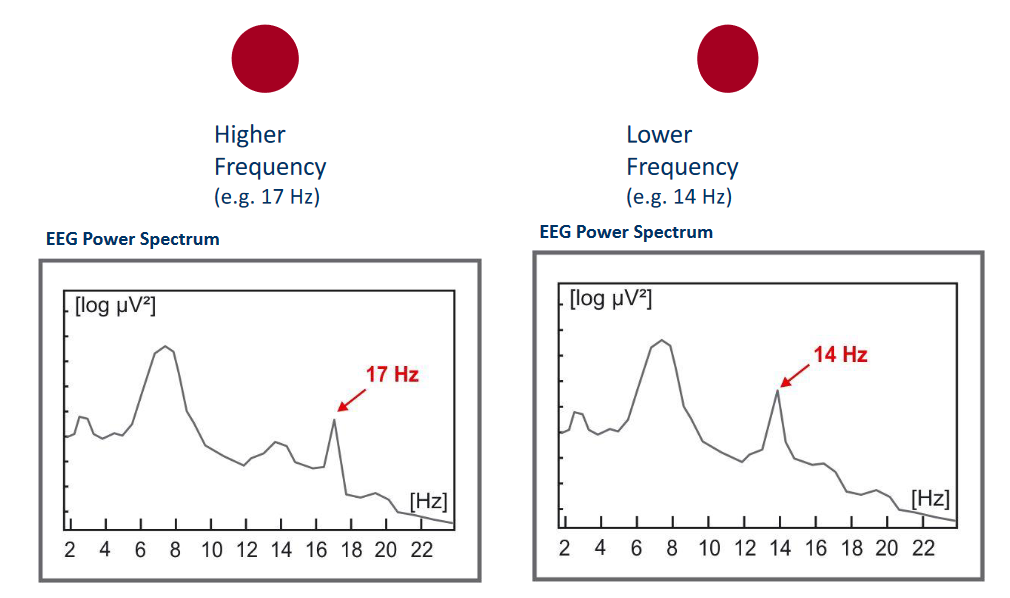
\includegraphics[scale=0.45]{gfx/SuI3_SSVEP_official.PNG} 
    \caption{Example usage of different flickering frequencies for SSVEP (based on \cite{IMG:SSVEP})}
    \label{def:SSVEP}
\end{figure}

\subsection{Spontaneous Potentials}
\label{sec:def:motim}

Spontaneous potentials, as mentioned before, can occur without the need of an external stimulus to be present \cite{martisius-2016}. They are recorded over a time span of a few seconds while brain activity is present in different frequencies (see Section \ref{sec:def:freqBand}) and in different regions of the brain. A combination of both a specific brain region and a specific frequency band can be attributed to a specific mental task (see Image \ref{def:SpontPot}) which then can be used to issue a specific command to the BCI \cite{martisius-2016}. 

\begin{figure}[h]
    \hspace*{-0.7cm}
    \centering
    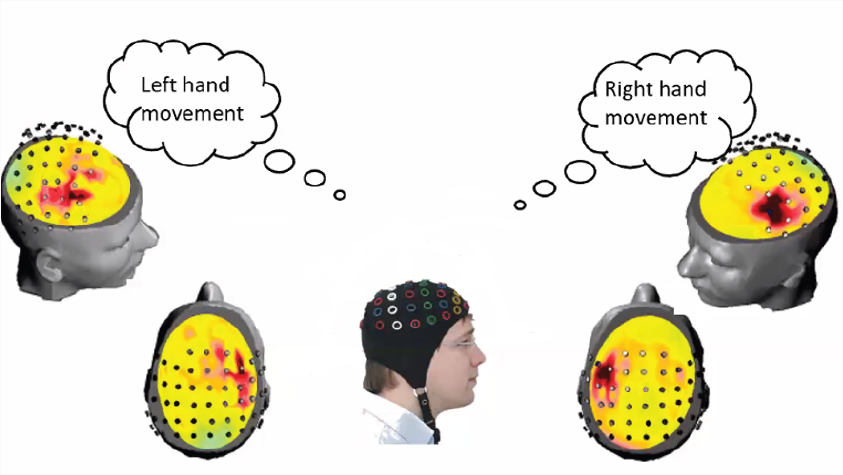
\includegraphics[scale=0.5]{gfx/SuI3_Spontaenous_potential.PNG} 
    \caption{Example of brain activity for specific mental tasks (based on \cite{IMG:SpontPot})}
    \label{def:SpontPot}
\end{figure}

\subsection{Motor Imagery (MI)}

Motor Imagery (MI) is a specific BCI paradigm in the category of spontaneous potentials, which uses the mental imagination of a movement without physically executing it. During MI, brain activity can be recorded in similar regions of the brain as during actual execution the movement, especially in areas of the sensorimotor cortex, where movement is planned and processed. % cite, is that clear and helpful for understanding?
These changes are commonly observed in the mu (8–13 Hz) and beta (13–30 Hz) frequency bands (see for reference Sec. \ref{sec:def:freqBand}) and are characterised by event-related desynchronisation (ERD) and event-related synchronisation (ERS), where the a change in power of specific frequency bands can be recorded, depending on the performed imagined movement task. % phrasing ok?

% might also take the picure from before in here and use a different one to symbolise spontaneous potentials (might be more clear)

In BCI applications, these signal changes can be detected and classified in order to translate imagined movements, such as imagining movement of the left or right hand, into control commands for external systems, like a game controller. % fitting?


% I think it's best to briefly describe the diferent paradigms here, especially P300, keep SSVEP and end with MI, where we just extend our already written section
% keep alphawow + butterfly game, omit neurosky, keep elden ring
\section{Neural Network architectures and algorithms}

Neural Networks (NNs) have been found to be useful in the use of classifying EEG data for their use for BCIs. % cite 
To get an understanding for the different types of NN used with BCI, especially in the examples presented in Chap. \ref{chap:relWork}, this section introduces the most common forms of NNs that can be used in BCI applications. % phrasing ok?

\subsection{Convolutional Neural Networks (CNNs)}

Convolutional Neural Networks (CNNs) are a type of NN that, while functioning similarly to classical NNs, are primarily
used for image processing \cite{oshea-2015}. % ciiiite
A distinctive feature of CNNs is that they can compute an output for an entire image region
using so-called “convolutional layers” (Convolutional rather than from each individual pixel, thereby significantly
reducing the number of parameters to be calculated \cite{oshea-2015}. % ciiiiiite (take the ones from our bachelor thesis)
% plus add a section how they can be used for our EEG data (extracting spatial and temporal features n stuff :3333, would fill this section + provide a bit of clarity about the terms so we don't have to specifically do a section for them cc:)


\subsection{Transformer}

% vvvvvvvvvvvv Translated stuff from our previous thesis: rephrase!
Transformers are based on the principle of \glqq attention\grqq, which enables the network to identify highly relevant parts of the input data and then highlight them. % cite!
In the case of translation, where the input sequential data consists of the words in the input sentence, attention would be helpful here to highlight words relevant to the context for the translation.

In the landmark paper \glqq Attention is all you need\grqq \space from 2017 \cite{vaswani-2017}, the Transformer was introduced as a model for sequence translation. This model, which, as was customary at the time, consisted of an encoder and a decoder connected by attention mechanisms, did, however, completely dispense with recurrences and convolutions for the first time.

Instead, the entire network architecture was based on attention mechanisms, thereby surpassing the performance of the previously best architectures for translation tasks.

Although a Transformer consists of both an encoder and a decoder, only the encoder of a Transformer will be examined in detail below, as it is the only component used in the architecture of the novel network architecture \acl{ViT}.

According to the paper, a Transformer's encoder consists of six stacked encoder layers, each composed of identical sublayers.

In the first sublayer, the input data is processed by a so-called ``multi-head self-attention” mechanism. Multi-head attention
is a concept for attention mechanisms in which the input data, instead of passing through a single attention layer, is processed in parallel through multiple attention layer and the results are subsequently combined and linearly mapped. Self-attention, in turn, is a mechanism that allows the remaining elements of the same sequence to be considered in the case of sequential data, thereby enabling contexts within the sequence to be identified and highlighted accordingly. The second part of the sublayer consists of a fully connected ``feed-forward network” that feeds the sequential input data from the ``multi-head self-attention” layer, regardless of their order, into the next, identically structured, encoder layer. At the end of each sublayer, the output data is normalized and added to the input data of the respective sublayer. % check + cite the correct paper!

% + add relevant picture if neeeded :3 (just have to see that it's not toooooooooo cmplex, as we only use transformer briefly in rel works and maybe as a possible approach, you got this :3)

% also add stuff about the decorder! (prob from the same paper)

% ^^^^^^^^^^^^^ reeeeeephraaaase :33333

\subsection{Common Spatial Patterns (CSP)}

Common Spatial Patterns (CSPs) is a spatial filtering method that is used in signal processing and is especially helpful in BCIs for extracting features from brain signals across multiple EEG channels. % cite? :,3
It was originally introduced by Koles et al. in their paper ``Spatial patterns underlying population differences in the background EEG” in 1990, where this method was proposed for analysing differences in EEG activity between different human populations \cite{koles-1990}.
Later, the approach was popularised and adapted for BCI applications by Ramoser et al. in the year 2000 by using subject-specific spatial filters for discriminating between left- and right-hand movement \cite{ramoser-2000}.% ciiiiite

\begin{figure}[h]
    \hspace*{-0.7cm}
    \centering
    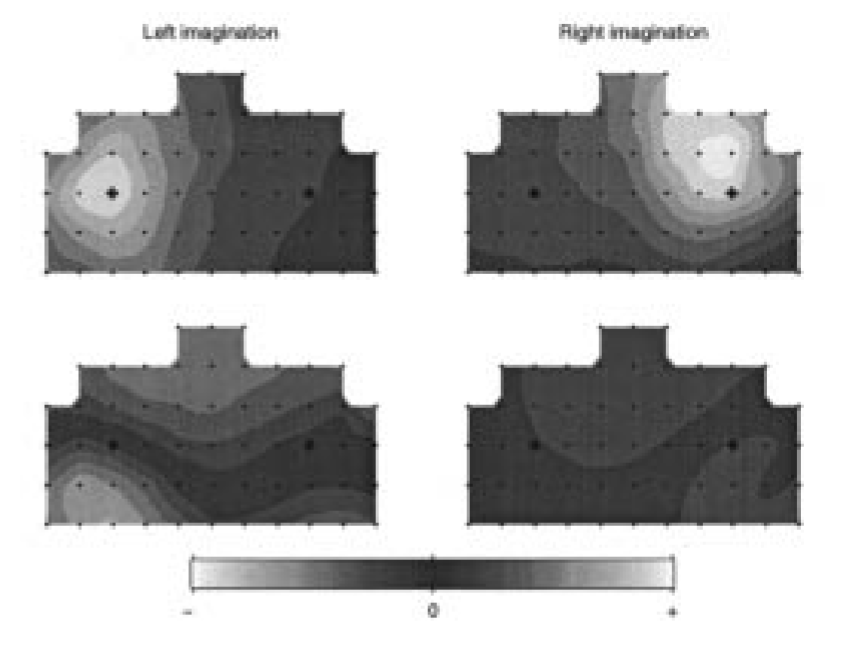
\includegraphics[scale=0.8]{gfx/MThes_CSPPatternVis.png} 
    \caption{Visualization of determined spatial filters for imagined left and right motor imagery across the EEG electrodes with lighter shading indicating high variance in that specific area (taken from \cite{ramoser-2000})} % is the description correct? should be well summarised
    \label{def:CSPVis}
\end{figure}

The method aims to find such filters which maximise the variance for one class of signals, like imagined left-hand movement while simultaneously minimising it for another class, like right-hand movement, thus aiding in increasing the separability between different MI tasks. Mathematically, this is achieved by computing covariance matrices for two signal classes and solving a generalised eigenvalue problem, % do we know what that is? :p
resulting in spatial filters that project the EEG signals into components with maximal discriminative variance differences (see for reference Img. \ref{def:CSPVis}) \cite{koles-1990}. % rephrase 'cause this is still heavily ChatGPT (or do we? It's really well written :,3) might just focuse on rewriting the last part of the sentence wiuth components n stuff
The extracted features can then be used as input for classification algorithms such as the ones presented in Chap. \ref{chap:relWork}.

% CSP are first and foremost a signal processing technique! (so not a 'real' pattern, sadly :,3)
% -> AI summary: Common Spatial Patterns (CSP) a supervised signal processing technique used to design spatial filters that maximize the variance (power) of electroencephalogram (EEG) signals for one motor imagery task while minimizing it for another. 


\section{Applications of BCI in gaming}
\label{chap:applications}


The following paragraphs present existing applications of BCIs in gaming, while also trying to showcase the usage of different BCI paradigms (see Chap. \ref{sec:def:paradigm}) used for controlling them. % might adapt and rephrase



\subsection{AlphaWoW by Nijholt et al.}

In 2009, Nijholt et al. published an article discussing the potential of using BCIs in gaming applications, giving examples for different already existing applications but also showing an application using BCI they developed themselves, which they called ``AlphaWoW'' \cite{nijholt-2009}. \emph{AlphaWoW} (see Fig. \ref{app:alphaWoW}), which is short for ``Alpha World of Warcraft'' is a BCI implementation developed for the Massive Multiplayer Role Playing Game \emph{World of Warcraft}, in which the player plays a character in a vast fantasy world, inhabited by other players' characters and characters controlled by the game system \cite{nijholt-2009}.

In this game, players can choose among different variations of characters to play which change their appearance and their abilities they can use to progress in the game. For the experiment, a Night-Elf Druid was chosen as the character to play the game, who has the ability to shape-shift themselves into a bear and back. Using a BCI, Nijholt et al. then made the transformation dependent on the users alpha brain wave activity (for reference see Chap. \ref{sec:def:freqBand}). While the player was relaxed and thus a high activity in the alpha range was being recorded, the player would remain in its Night-Elf Druid form. Once the BCI detected low activity in the alpha range, meaning that the player was less relaxed, more alert and experiencing stress, the BCI made the character shape-shift into its bear form \cite{nijholt-2009}.


\begin{figure}[h]
    \hspace*{+0.3cm}
    \centering
    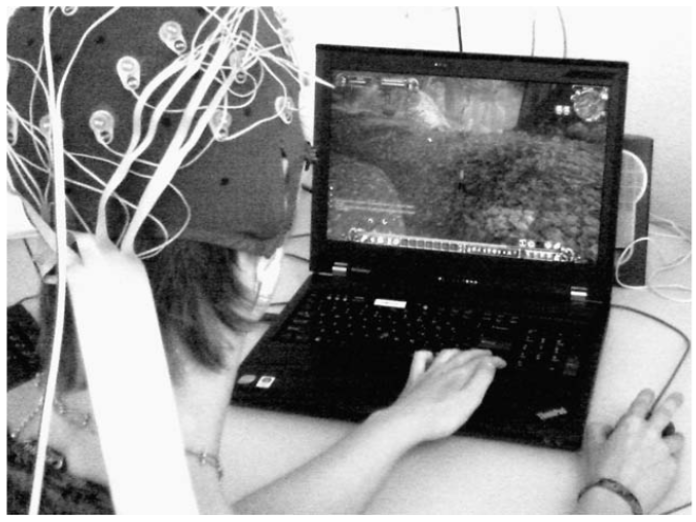
\includegraphics[scale=0.5]{gfx/SuI3_AlphaWoW.PNG} 
    \caption{User playing World of Warcraft using mouse, keyboard and the BCI developed by Nijholt et al. \cite{nijholt-2009}} % rephrase?
    \label{app:alphaWoW}
\end{figure}

Both forms had their advantages for managing enemies in the game. In bear form, the player had increased durability while also dealing high close range combat damage and in Night-Elf druid form, the player could manage dealing with enemies form afar with ranged spells but also had significantly less durability. Most importantly, only while in Night-Elf Druid form, the player was able to heal themselves should they have taken damage in combat with enemies. Thus, the player had to learn to use the BCI to their advantage, relaxing themselves when they wanted to heal themselves and battling enemies form afar and stressing themselves if they wanted to switch to the Night-Elf Druid's bear form for strategical reasons. Using this application, Nijholt et al. noted, the users got satisfaction out of the challenge of having to incorporating this system into their gameplay, showing a possible use of different brain wave ranges for controlling specific action inside a game \cite{nijholt-2009}.

\subsection{Character Controller using SSVEPs through in-game objects}
\label{sec:app:butterfly}

In the context of a game, just having flashing lights at different frequencies to record SSVEPs for a BCI might be off-putting, potentially decreasing the immersion into it. A possible solution to integrate SSVEP triggers into a game in a more natural way was shown in a paper by Legény et al. in 2011 where they presented an SSVEP-based BCI which allowed the user to control their movement in a Virtual Reality (VR) environment in their own pace \cite{legeny-2011}.

For general navigation, three butterflies were constantly shown on the screen, flapping their wings at different frequencies and each corresponding to a direction of movement throughout the virtual space (see Fig. \ref{app:butterflies}). Additionally, to give the user real-time feedback on whether their concentration on a butterfly was successful or not, the BCI would make the antennas of a specific butterfly cross, if it detected focus on that exact butterfly and make the antennas go further apart when sensing that the user was not concentrating on that specific butterfly.
Therefore, to move through the virtual space, the user first had to focus on a butterfly representing the movement direction of their choice and then keep concentrating on it. As long as the BCI recorded concentration on that specific butterfly, it would continuously move the user in that direction until the concentration was either lost or the BCI recorded that another butterfly was being focused on.

\begin{figure}[h]
    \hspace*{-1.0cm}
    \centering
    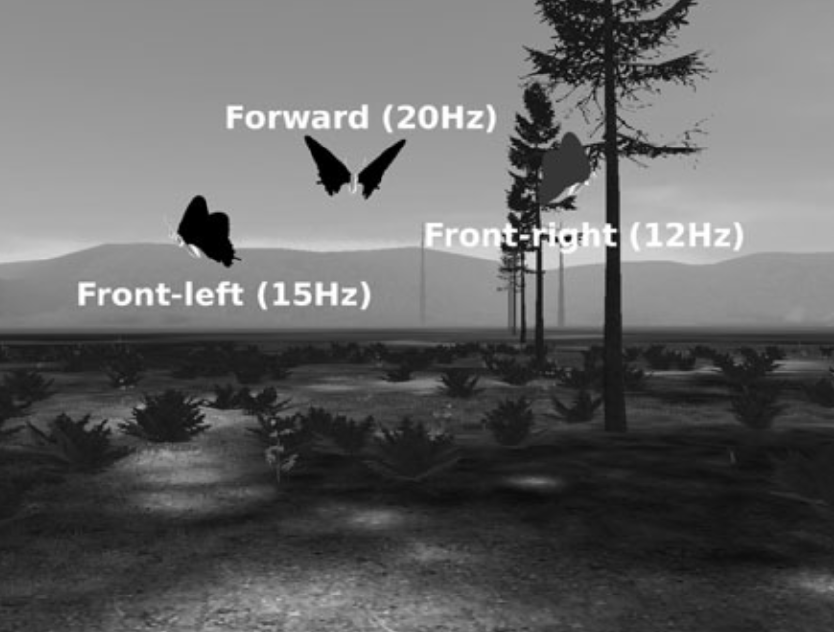
\includegraphics[scale=0.5]{gfx/SuI3_SSVEP_butterflies.PNG} 
    \caption{Butterflies flapping wings at different frequencies for character control in a virtual space using SSVEPs \cite{legeny-2011}}
    \label{app:butterflies}
\end{figure}

The BCI was then tested in an experiment, which aimed to analyse movement performance against movement with keyboard and mouse as well as analysing subjective criteria of the participants, like the feeling of presence in the given virtual world, using both the character controller (i.e. the butterflies flapping their wings) and its real-time feedback (i.e. the crossing antennas). In the same experiment, the butterfly overlay was also compared to a classic SSVEP overlay with flickering lights.
The participants were first asked to complete a training session, where they learned to use the BCI and calibrated the classifier of the BCI which was identifying in what direction the users wanted to move. After training, they were asked to move their character, which was shown in a VR world set in a virtual forest, around five trees to cross a finish line at the end. Additionally, they were given a time limit of eight minutes to complete the slalom trial.

Aside from the expected observation that movement using keyboard and mouse was significantly faster than movement using the BCI, results showed that more than half of the participants were able to complete the trial inside the given time limit of eight minutes. Moreover, results showed that, during the trial, participants were feeling more present in the virtual space using the butterflies for their movement control as opposed to moving through the virtual forest using a classic SSVEP overlay with flickering lights.

\subsection{Emulating a controller using BCIs}

A rather recent example for using a hybrid BCI controller for gaming is presented by the ``video-game and variety streaming-video broadcaster'' \cite{nolan-2023} Perri Karyal \cite{nolan-2023}.
Karyal developed a hybrid BCI controller using a 14-channel headset (see Fig. \ref{chall:emotiv}) for playing the game \emph{Elden Ring}, released in 2022, in which a character moves through an open world and defeats enemies to reach the end of the game's story. Using this headset she was able to issue mental commands that would be translated into attack (see Fig. \ref{out:perri}), spell casting or dodge actions inside the game by having certain mental visualisations of the commands, thus evoking  spontaneous potentials in the brain (for reference, see Chap. \ref{sec:def:spont}). 

\begin{figure}[h]
    \hspace*{-0.2cm}
    \centering
    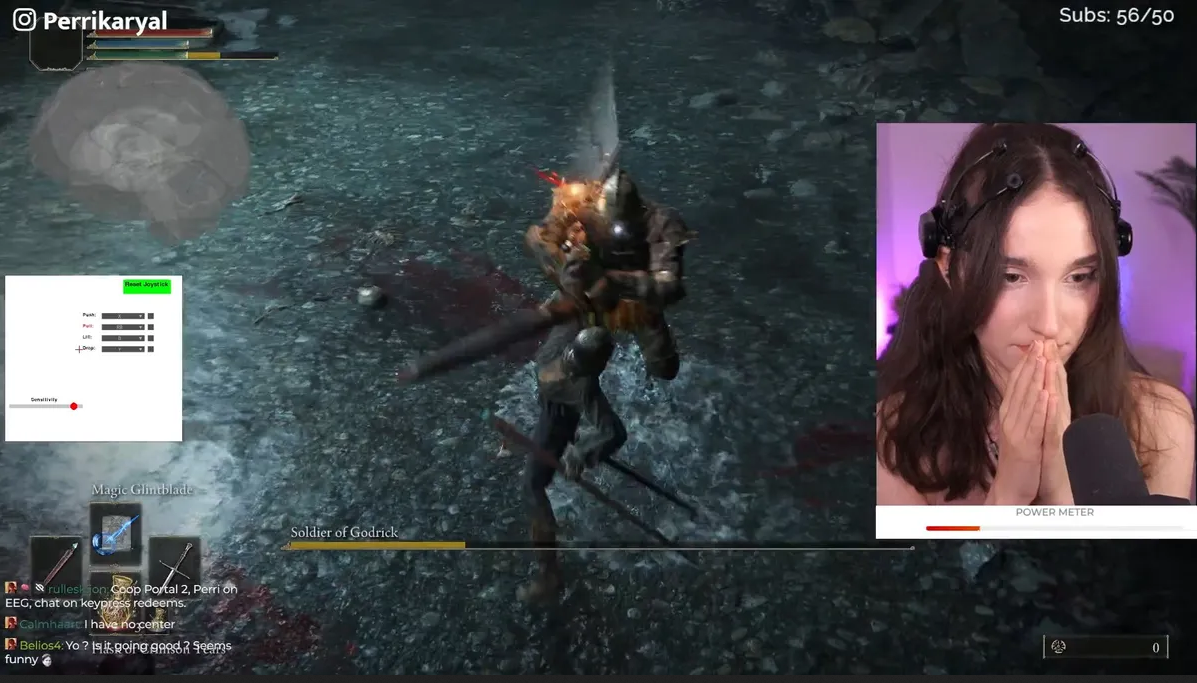
\includegraphics[scale=0.45]{gfx/SuI3_perri_karyal.PNG} 
    \caption{Stream screenshot showing Karyal playing \emph{Elden Ring} where the attack command has just been detected by her BCI (taken from \cite{nolan-2023})} % rephrase?
    \label{out:perri}
\end{figure}


As an example, in order to issue the attacking command inside the game, Karyal would visually imagine ``pushing something forward in [her] head'' \cite{nolan-2023}, which would increase brain activity in a specific region of the brain which could then be detected by the BCI to issue that specific command. By using additional head-tracking for movement she was later able to create a full hands-free controller for that game \cite{nolan-2023}.
While this recent development looks promising for future applications of BCIs in modern games, Karyal herself stated, that in order for the BCI to recognise the commands as accurately as possible (and as shown in her videos), she had to spend more than 250 hours just for calibrating the headset to her mental visualisations \cite{nolan-2023}, bringing us back to the issue of training, one of the main challenges of using BCIs in gaming applications (see Chap. \ref{chall:training} for details).

\section{Relevant challenges}
\label{chap:challenges}


% might also have to restructure this chapter to be more understnading and in line with our actuial thesis goal

The usage of BCIs in gaming applications, however, comes with its own extensive set of challenges. In this paragraph, they are summarised under the most important aspects, while trying to give both concrete examples for their issues in gaming applications and also proposing possible solutions for them, where possible.

% mention that BCI, for now, probably will never be able to be used in fast-pced settings like action games (actually  might put that into conclusions! could be interesting)

\subsection{Signal Quality} % section relevant?

The first challenge for using BCI headsets in gaming applications can be found in the quality of the signal recorded from the brain activity itself. As mentioned in Chap. \ref{sec:def:invasive}, an electrode placed directly inside the brain would ensure optimal signal acquisition, yet this approach is definitely not suitable for making BCI games for a large number of users in a non-clinical setting.
Therefore, the examples for BCIs presented in Chap. \ref{chap:applications} are exclusively non-invasive, coming with the advantage of not requiring surgery for their use while accepting the loss in signal quality which comes with it. 
Signal quality is also affected by the number of electrodes used for its acquisition. Generally, the more electrodes (also called ``channels'') are placed on the head (going up to 256 channels \cite{seeck-2017}), the higher the resolution of the recorded signal can be. According to the International Federation of Clinical Neurophysiology (IFCN), the standard amount of channels for recording brain signals in clinical settings was once 32 channels in 1998 but was then updated to 25 channels in 2017 \cite{nuwer-1998, seeck-2017}. % rephrase to reduce mental load reading this? might omit the 256 electrode part or just say hey the standard is 25 deal with ii
BCIs in non-clinical settings use considerably fewer channels, like the SSVEP controller presented in Chap. \ref{sec:app:butterfly}, which uses six channels and thus decreases the overall quality of the signals that can be recorded by them.
A reason for that reduction is that the more channels are present, the more time is required to set up the BCI for the user, especially using wet electrodes (see Chap. \ref{def:bciNonInv} for details), and the more the BCI itself costs. To compromise that, BCIs sold commercially use fewer channels and dry electrodes (see Fig. \ref{chall:emotiv}), reducing setup time but potentially also decreasing their signal quality compared to BCIs in clinical settings.

\begin{figure}[h]
    \hspace*{-0.0cm}
    \centering
    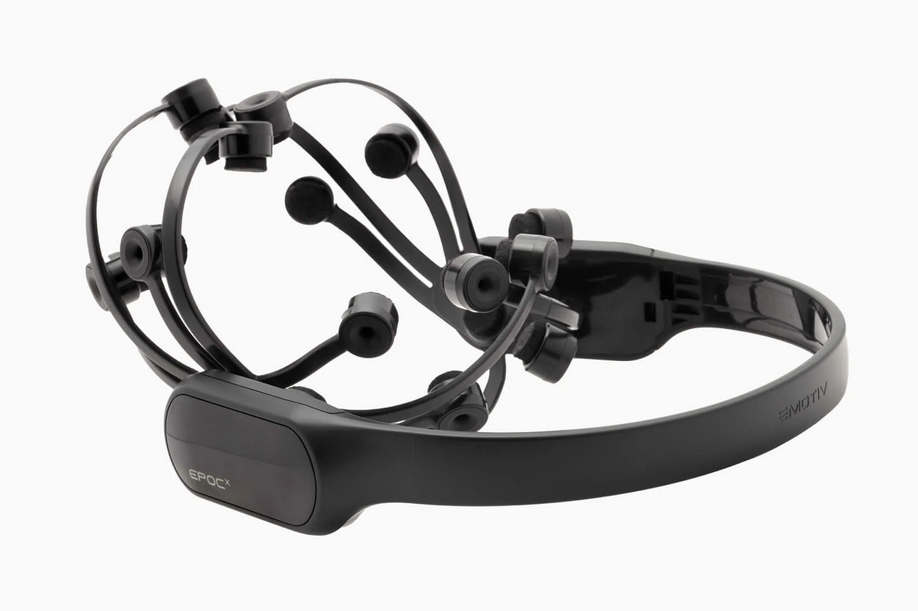
\includegraphics[scale=0.3]{gfx/SuI3_emotif_epoc.PNG} 
    \caption{A 14-channel headset for brain signal acquisition sold by \emph{EMOTIV} (taken from \cite{EMOTIV:EpocX})}
    \label{chall:emotiv}
\end{figure}

[Go into more detail here!] % might also mention the issues in otur actual implementation chapter and note how we solved the issues and which algrotihms we used in order to do so
Additionally, signal quality in non-invasive BCIs is further decreased with error sources such as head, eye and muscle movement of the user (mentioned in Chap. \ref{sec:def:non-invasive}). To reduce that kind of loss in signal quality and to increase the reliability of BCI to correctly translate brain signals into potential control commands, the incoming signals can be filtered using a range of different methods including those frequently used in machine learning % can go into a bit more detail here, since we do write our master thesis
\cite{abdulkader-2015}.


\subsection{Transfer Rate}

% insert the image about transfer rate here (if it still exists and we find it)

Another issue in using BCIs in gaming applications is their low transfer rates of issued mental commands to evoke action on the screen, especially compared to the transfer rate of a keyboard and mouse. 
For BCIs, the transfer rate can be derived from the Information Transfer Rate (ITR), which is used as a metric to assess a combination of the BCIs selection time, number of choices and recognition accuracy \cite{yadav-2020}. For evoked potentials that use an external stimulus, like the SSVEP, the ITR ranges between 60 and 100 bits per minute \cite{yadav-2020} meaning that one bit of information can be transferred approximately every 0.75 seconds, whereas keyboards take around 0.05 to 0.1 seconds to transfer information about a key press \cite{casiez-2017, wimmer-2019}. The time difference in using SSVEPs compared to a keyboard was further shown in the SSVEP controller by Legény et al. (shown in Chap. \ref{sec:app:butterfly}), where the authors reported, that the users were able to complete the virtual slalom course four to seven times faster on keyboard then they did using the SSVEP controller \cite{legeny-2011}.

This could pose a problem for the application of BCIs in fast-paced games like shooters or others action games. A possible solution for that might be either choosing to develop BCI games with less time-critical game elements or using a hybrid input system which uses both BCI input and traditional input like keyboard and mouse or touch, as seen in \emph{AlphaWoW} and specifically Karyals BCI controller for \emph{Elden Ring}, which serves as a defining inspiration for the BCI controller used in this thesis for the evaluation of our different calibration algorithms.

\subsection{Training}
\label{chall:training}

The last major and, in the context of using BCIs in gaming applications, most pressing issue is the significantly high time needed to train BCIs. 
In order for the BCI to correctly and rapidly translate the brain signal inputs of a user to a corresponding action, the BCI has to be extensively calibrated to the inputs of the user. Additionally, the user also has to spend some time to figure out how to support the BCI in the classification of their signals, for example by focusing on being relaxed to make it easier for the system to detect activity in alpha range or choosing mental commands % defintiely reference mental commands in spontaneous potentials too and refere to the EMOTIV site for mental commands (as long as they somehow are backed by science, could always say, that they are called mental commands by some companies and insitutions producing/manufacturing BCI)
that are easier detected by the BCI. Thus, in a way, both the BCI and its user have to undergo some form of calibration to learn to ``understand'' each other in order for the BCI to function properly and accurately \cite{nijholt-2009}.

Generally speaking, the more time is spent training the BCI and its user, the more precise the results can be \cite{nijholt-2009}. 
However, in gaming applications, this extended training time might be bothersome to perform before even playing the game, resulting in a barrier for playing games that use BCIs for controlling it. For that reason, Nijholt et al., in their paper ``Turning Shortcomings into Challenges: Brain-Computer Interfaces for Games'', suggested integrating BCI calibration directly into the game (e.g. by using an in-game tutorial before the actual game) \cite{nijholt-2009}. Nijholt et al. also mention, that this definitely asks game designers to incorporate adequate levels and game elements requiring BCI control to be solved successfully into their games to enable such form of integrated calibration \cite{nijholt-2009}. 
This represents the main underlying issue of using BCIs in video games which the algorithms presented and used in this thesis aim to minimise and contain. % prob def rephrase xd
% might close the challenges subsection with a transition to 

[also mention inter-session + inter-subject variability here!]
[-----------]

[Now follows the intro to the technical stuff like the specific algorithms, Neural Networks, CNN,etc!]

Current stuff:

CNN?
Transformer % yes! Will have to explain both CNN and Transformer briefly


[----------]

(but also stuff like temporal resolution and all the stuff that might be new in the related work so people understand what we're actually talking about CC:)

% also might have to restructure afterwards if needed uwu

% might actually also use stuff from our bachelorthesis if we talk about different networks like CNN n stuff

% vvv will be needed once we definitely know which kind of algorthims we will use, so it's wise to just wait for thesis progression in order to exactly know what needs to be defined still
% might need to think about defining algorithm stuff too, depending on what they entail, might also ask Guthe about it if we should also introduce the readers to neural nets or if that's a given once you are in this field already (might actually be redundant since we come from comp science), might think about defining specific parts of the algorithm if they go above and beyonf the 'classic' neural network stuff                                                                                                                                                                                                                                                                                                                                                                                                                                                                                                                                                                                                                                                                                                                                                                                                                                                                                                                                                                                                        